\section{Results}
\label{sec:results}

We benchmark our implementation by measuring the time taken to generate proofs for the setup phase of the game. We first compare the na{\"\i}ve design with the Merkle tree implementation and subsequently benchmark them across varying numbers of ship coordinates. The benchmarks in this section were run on the following machine specifications:

\begin{itemize}
    \item \textbf{\Gls{os}} \--- Arch Linux (Linux kernel 6.19.11-arch1-1).
    \item \textbf{\Gls{cpu}} \--- Intel Core Ultra 7 155U, 14 cores, up to $\qty{4.8}{\giga\hertz}$.
    \item \textbf{Memory} \--- $\qty{16}{\gibi\byte}$.
\end{itemize}

\cref{fig:executionTimesNaive,fig:executionTimesMerkle,fig:executionTimesComparison} show proof generation times with each data point being the mean of one hundred independent runs. To facilitate the scaling and maintain a uniform benchmark, we have simplified the circuit logic by relaxing the standard Battleship schema. Rather than enforcing the traditional multiset of ship lengths from \cref{eq:L}, the circuit allows for arbitrary ship lengths. To illustrate, consider a board that has 23 coordinates. Then, the multiset $\mathcal{L}$ from \cref{eq:L} is defined as $\set{10, 10, 3}$, which fills from the upper left corner in a left\-/to\-/right manner. In addition, the benchmarking starts at two ship coordinates to ensure the overlap check is not optimized out of the circuit.

\subsection{Na{\"\i}ve Approach}
\label{subsec:naiveApproach}

Recall from \cref{subsec:zkFriendly,subsec:merkle} that the na{\"\i}ve approach has a hard upper bound of seven coordinates. Hence, we are only able to analyze the results by varying the number of ship coordinates from two to seven, inclusively. The circuit for two coordinates is shown in \cref{lst:initialProofCircuitNaiveA,lst:initialProofCircuitNaiveB,lst:initialProofCircuitNaiveC}, with minor modifications for the other number of ship coordinates as described in \cref{subsec:initialProofCircuit}. The results of the measurements are shown in \cref{fig:executionTimesNaive}. As previously noted, the proving time scales linearly in the number of inputs, and that trend is apparent in the figure. Although the number of coordinates remains fixed in the standard game of Battleship, as described in \cref{subsec:battleship}, this structural limitation renders the na{\"\i}ve design unsuitable for other \gls{p2p} games with larger state spaces. The proving time would be prohibitively slow for the end\-/users. In addition, notice that the proving time for only two ship coordinates is $\qty{860}{\milli\second}$. This behavior suggests that the total execution time is dominated by a significant constant overhead that is independent of the number of ship coordinates. This overhead likely stems from at least one of the following:
\begin{itemize}
    \item \textbf{Initialization costs} \--- Setting up the circuit environment.
    \item \textbf{Fixed verification steps} \--- Certain cryptographic constraints or proof generation steps that must be processed regardless of the specific input size.
    \item \textbf{System latency} \--- Basic \gls{io} and processing cycles inherent to the benchmarking environment.
\end{itemize}

\begin{figure}
    \centering
    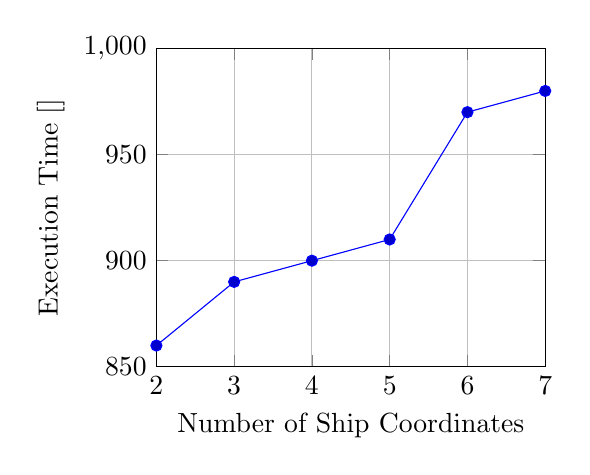
\begin{tikzpicture}
        \begin{axis}[
            grid=major,
            height=16em,
            xlabel={Number of Ship Coordinates},
            ylabel={Execution Time [$\unit{\milli\second}$]},
            xmin=2,
            xmax=7,
            xtick={2,3,...,7},
            ymin=0.85,
            ymax=1.0,
            y coord trafo/.code={
                \pgfmathparse{#1*1000}\pgfmathresult
            },
        ]
            \addplot+ coordinates {
                (2,0.86)
                (3,0.89)
                (4,0.90)
                (5,0.91)
                (6,0.97)
                (7,0.98)
            };
        \end{axis}
    \end{tikzpicture}
    \caption{Analyzing performance in the na{\"\i}ve approach.}
    \label{fig:executionTimesNaive}
\end{figure}

\subsection{Merkle Tree Approach}

The execution times for different numbers of ship coordinates for variations of the circuit displayed in \cref{lst:initialProofCircuitMerkleA,lst:initialProofCircuitMerkleB,lst:initialProofCircuitMerkleC,lst:initialProofCircuitMerkleD}, still adapted to the number of ship coordinates as described in \cref{sec:initialProofCircuit}, are illustrated in \cref{fig:executionTimesMerkle}. As shown in the plot, the execution time exhibits a shallow growth curve as the number of ship coordinates increases from only two to filling the entire ten\-/by\-/ten board at one hundred. Although a slight upward trend is visible, moving from approximately $\qty{267}{\milli\second}$ at the lower bound to roughly $\qty{281}{\milli\second}$ at the upper bound, the increase is not proportional to the fiftyfold increase in the number of ship coordinates. This can be attributed to the fact that the verification time of a Merkle tree scales logarithmically, as discussed in \cref{subsec:merkle}.

Furthermore, the data exhibit minor fluctuations, such as the notable dip at eleven ship coordinates. However, since the range across the entire data set is so small, the system demonstrates excellent scalability within this specific parameter range, indicating that the incremental cost of adding one ship coordinate to the circuit is negligible compared to the base cost of the operation itself. Also note that there is a constant overhead as in \cref{subsec:naiveApproach}, which stems from the same reasons stated there.

\begin{figure}
    \centering
    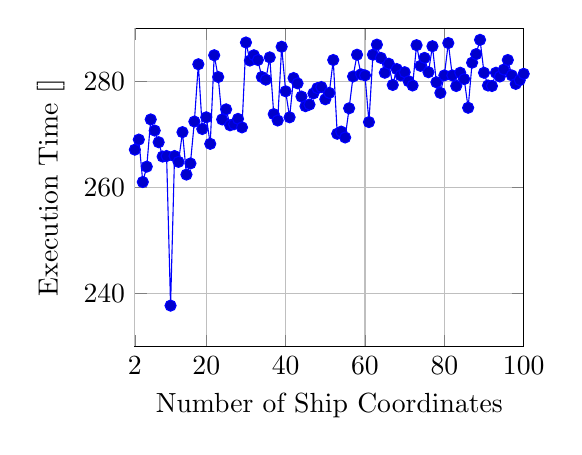
\begin{tikzpicture}
        \begin{axis}[
            grid=major,
            height=16em,
            xlabel={Number of Ship Coordinates},
            ylabel={Execution Time [$\unit{\milli\second}$]},
            xmin=2,
            xmax=100,
            ymin=0.23,
            ymax=0.29,
            extra x ticks={2},
            y coord trafo/.code={
                \pgfmathparse{#1*1000}\pgfmathresult
            },
        ]
            \addplot+[color=blue] coordinates {
                (2,0.2671)
                (3,0.2690)
                (4,0.2610)
                (5,0.2639)
                (6,0.2728)
                (7,0.2707)
                (8,0.2685)
                (9,0.2658)
                (10,0.2659)
                (11,0.2377)
                (12,0.2659)
                (13,0.2648)
                (14,0.2704)
                (15,0.2624)
                (16,0.2645)
                (17,0.2724)
                (18,0.2832)
                (19,0.2710)
                (20,0.2732)
                (21,0.2682)
                (22,0.2849)
                (23,0.2808)
                (24,0.2728)
                (25,0.2747)
                (26,0.2717)
                (27,0.2719)
                (28,0.2729)
                (29,0.2713)
                (30,0.2873)
                (31,0.2839)
                (32,0.2849)
                (33,0.2840)
                (34,0.2808)
                (35,0.2803)
                (36,0.2845)
                (37,0.2738)
                (38,0.2726)
                (39,0.2865)
                (40,0.2781)
                (41,0.2732)
                (42,0.2806)
                (43,0.2796)
                (44,0.2771)
                (45,0.2753)
                (46,0.2756)
                (47,0.2777)
                (48,0.2787)
                (49,0.2789)
                (50,0.2766)
                (51,0.2778)
                (52,0.2840)
                (53,0.2701)
                (54,0.2705)
                (55,0.2694)
                (56,0.2749)
                (57,0.2809)
                (58,0.2850)
                (59,0.2813)
                (60,0.2811)
                (61,0.2723)
                (62,0.2850)
                (63,0.2869)
                (64,0.2844)
                (65,0.2816)
                (66,0.2833)
                (67,0.2793)
                (68,0.2823)
                (69,0.2811)
                (70,0.2817)
                (71,0.2800)
                (72,0.2792)
                (73,0.2868)
                (74,0.2829)
                (75,0.2844)
                (76,0.2817)
                (77,0.2866)
                (78,0.2798)
                (79,0.2778)
                (80,0.2811)
                (81,0.2872)
                (82,0.2811)
                (83,0.2791)
                (84,0.2816)
                (85,0.2804)
                (86,0.2750)
                (87,0.2835)
                (88,0.2851)
                (89,0.2878)
                (90,0.2816)
                (91,0.2792)
                (92,0.2791)
                (93,0.2816)
                (94,0.2809)
                (95,0.2822)
                (96,0.2840)
                (97,0.2811)
                (98,0.2795)
                (99,0.2802)
                (100,0.2814)
            };
        \end{axis}
    \end{tikzpicture}
    \caption{Analyzing performance in the Merkle tree approach.}
    \label{fig:executionTimesMerkle}
\end{figure}

\subsection{Comparison of Approaches}

Since the circuit in the na{\"\i}ve approach is bounded by a hard limit of at most seven ship coordinates, as discussed in \cref{subsec:zkFriendly}, comparisons in \cref{fig:executionTimesComparison} are made across these values. The first point of comparison would be the linear versus logarithmic scaling exhibited in the plots. As noted, the Merkle tree circuit scales better than the na{\"\i}ve implementation, even for a small number of ship coordinates.

In summary, the Merkle tree approach scales better in our implementation. Even if the na{\"\i}ve implementation offered superior performance, it remains practically infeasible because a standard game requires more than seven ship coordinates.

\begin{figure}
    \centering
    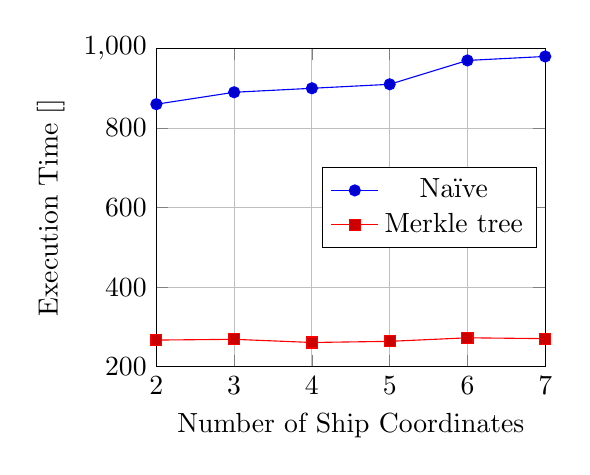
\begin{tikzpicture}
        \begin{axis}[
            grid=major,
            height=16em,
            legend style={at={(0.98,0.5)},anchor=east},
            xlabel={Number of Ship Coordinates},
            ylabel={Execution Time [$\unit{\milli\second}$]},
            xmin=2,
            xmax=7,
            xtick={2,3,...,7},
            ymin=0.2,
            ymax=1.0,
            y coord trafo/.code={
                \pgfmathparse{#1*1000}\pgfmathresult
            },
        ]
            \addplot+ coordinates {
                (2,0.86)
                (3,0.89)
                (4,0.90)
                (5,0.91)
                (6,0.97)
                (7,0.98)
            };
            \addlegendentry{Na{\"\i}ve}
            \addplot+ coordinates {
                (2,0.2671)
                (3,0.2690)
                (4,0.2610)
                (5,0.2639)
                (6,0.2728)
                (7,0.2707)
            };
            \addlegendentry{Merkle tree}
        \end{axis}
    \end{tikzpicture}
    \caption{Comparing performance in the na{\"\i}ve and Merkle tree approaches.}
    \label{fig:executionTimesComparison}
\end{figure}
